%Master File:lectures.tex
\lesson{Inner Product Spaces}
\vspace{-2cm}
\begin{center}
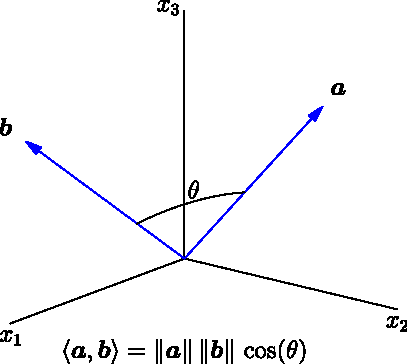
\includegraphics[width=0.6\linewidth]{inner_product}
\end{center}
\keywords{Inner products, operators}

%%%%%%%%%%%%%%%%%%%%%%% Next Slide %%%%%%%%%%%%%%%%%%%%%%%
\renewcommand{\Outline}{%
\begin{slide}
\section[1]{Outline}

\begin{minipage}{12cm}
  \begin{enumerate}\squeeze
    \outlineitem{Inner Products}{innerproduct}
    \outlineitem{Operators}{operators}
  \end{enumerate}
\end{minipage}\hfill
\begin{minipage}{10cm}
  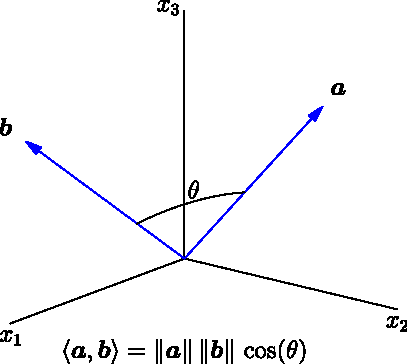
\includegraphics[height=10cm]{inner_product}
\end{minipage}
\end{slide}
\addtocounter{outlineitem}{1}
}

\setcounter{outlineitem}{1}

%%%%%%%%%%%%%%%%%%%%%%% Next Slide %%%%%%%%%%%%%%%%%%%%%%%
\Outline % Inner product
\toptarget{firstoutline}
%%%%%%%%%%%%%%%%%%%%%%% Next Slide %%%%%%%%%%%%%%%%%%%%%%%

\begin{slide}
\section{Recap}

\begin{PauseHighLight}
  \begin{itemize}
  \item We have looked at vector space\pause{} (closed sets where we can add
    elements and multiply them by a scalar)\pauseb
  \item Recall that vector spaces don't just apply to normal vectors
    ($\mathbb{R}^n$), but to matrices, functions, sequences, random
    variables, \ldots\pause
  \item Proper distances or metrics, $d(\bm{x}, \bm{y})$, allow us to
    construct ideas about geometry of the vector space\pause
  \item Norms, $\len{\bm{x}}$, that allow us to reason about the size of vector\pause
  \item Norm induce a distance, $d(\bm{x}, \bm{y}) = \len{\bm{x}-\bm{y}}$\pause 
  \end{itemize}
\end{PauseHighLight}

\end{slide}



%%%%%%%%%%%%%%%%%%%%%%% Next Slide %%%%%%%%%%%%%%%%%%%%%%%

\begin{slide}
\section[-1]{Inner Products}

\begin{PauseHighLight}
  \begin{itemize}
  \item We will often consider objects with an \textit{inner product}\pause
  \item For vectors in $\mathbb{R}^n$
    \begin{align*}
      \langle \bm{x}, \bm{y} \rangle = \bm{x}^\tr\bm{y} = \sum_{i=1}^n
      x_i\,y_i \pause
    \end{align*}
  \item For functions\vspace*{-1em}
    \begin{align*}
      \langle f, g \rangle = \int_{x\in\mathcal{I}} f(x)\,g(x)\,\dd x\pause
    \end{align*}
  \item For $m \times n$ matrices\vspace*{-1em}
    \begin{align*}
      \inner{\mat{A}}{\mat{B}} = \mathrm{Tr} \, \mat{A}^\tr \mat{B} =
      \sum_{i=1}^m \sum_{j=1}^n A_{ij} B_{ij}\pause
    \end{align*}
  \end{itemize}
\end{PauseHighLight}

\end{slide}

%%%%%%%%%%%%%%%%%%%%%%% Next Slide %%%%%%%%%%%%%%%%%%%%%%%

\begin{slide}
\section[-1]{Axioms of Inner Products}

\begin{PauseHighLight}
  \begin{itemize}
  \item An inner product satisfies
      \begin{enumerate}\squeeze
      \item $\inner{\bm{x}}{\bm{x}} \geq 0$ for all $\bm{x}\in\mathcal{V}$\pause
      \item $\inner{\bm{x}}{\bm{x}} = 0$  if and only if $\bm{x}=\bm{0}$\pause
      \item $\inner{\alpha\, \bm{x}}{\bm{y}} = \alpha\,
        \inner{\bm{x}}{\bm{y}}$\pause
      \item $\inner{\bm{x}}{\bm{y}+\bm{z}} = \inner{\bm{x}}{\bm{y}} +
        \inner{\bm{x}}{\bm{z}}$\pause
      \item $\inner{\bm{x}}{\bm{y}} = \inner{\bm{y}}{\bm{x}}$\pause
      \end{enumerate}
    \item We can show that $\len{\bm{x}} = \sqrt{\inner{\bm{x}}{\bm{x}}}$
      satisfies the axioms of a norm, so that an inner-product space is
      a normed space\pause
    \item The norm associated with the inner-product for vectors in
      $\mathbb{R}^n$ (i.e. $ \langle \bm{x}, \bm{y} \rangle =
      \bm{x}^\tr\bm{y}$) is the Euclidean norm $\|\bm{x}\| = \sqrt{\bm{x}^\tr\bm{x}}$\pause
  \end{itemize}
\end{PauseHighLight}

\end{slide}

%%%%%%%%%%%%%%%%%%%%%%% Next Slide %%%%%%%%%%%%%%%%%%%%%%%

\begin{slide}
\section{Cauchy-Schwarz Inequality}

\begin{PauseHighLight}
  \begin{itemize}
  \item One of the most important results of inner-product spaces,
      known as the \emph{Cauchy-Schwarz inequality} is that
      \begin{align*}
        \inner{\bm{x}}{\bm{y}}^2 \leq \inner{\bm{x}}{\bm{x}} \,
        \inner{\bm{y}}{\bm{y}} = \len{\bm{x}}^2\,\len{\bm{y}}^2\pause
      \end{align*}
    \item Or
      \begin{align*}
         | \inner{\bm{x}}{\bm{y}}| \leq   \len{\bm{x}}\,\len{\bm{y}}\pause
      \end{align*}
    \item This is a very general result so for example
      \begin{align*}
        \left| \int  f(x)\,g(x) \dd x \right| \leq  \sqrt{\bra{\int f^2(x)\,
        \dd x} \bra{\int g^2(x)\, \dd x}}\pause
      \end{align*}
  \end{itemize}
\end{PauseHighLight}
  

\end{slide}


%%%%%%%%%%%%%%%%%%%%%%% Next Slide %%%%%%%%%%%%%%%%%%%%%%%

\begin{slide}
\section[-2]{Angles Between Vectors}

\begin{PauseHighLight}
  \begin{itemize}
  \item A natural interpretation of the inner product is in providing a
    measure of the angle between vectors\pause
    \begin{center}
      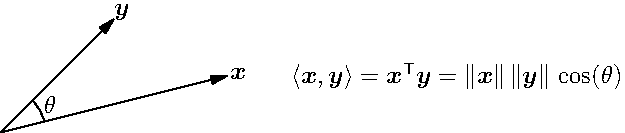
\includegraphics[width=0.9\linewidth]{inner_product_1}
    \end{center}
  \item Vectors are orthogonal if $\langle \bm{x}, \bm{y} \rangle = 0$\pause
  \item We can extend this idea to functions
    \begin{align*}
      \langle f(x), g(x) \rangle = \int_{x \in \mathcal{I}}
      f(x)\, g(x) \dd x = \|f(x)\| \, \|g(x)\|\, \cos(\theta)\pause
    \end{align*}
  \item Note that $\sin(x)$ and $\cos(x)$ are orthogonal in the interval
    $[0,2\,\pi]$\pause
  \end{itemize}
\end{PauseHighLight}


\end{slide}

%%%%%%%%%%%%%%%%%%%%%%% Next Slide %%%%%%%%%%%%%%%%%%%%%%%

\begin{slide}
\section[-2]{Basis Functions}

\begin{PauseHighLight}
  \begin{itemize}
  \item Any set of vectors $\{\bm{b}_i|i=1,\ldots\}$ that span the space
    can be used as a basis or coordinate system\pause
  \item The simplest and most useful case is when the vectors are
    orthogonal and normalised (i.e. $\|\bm{b}_i\|=1$)\pause
  \item In $\mathbb{R}^3$ we could use $\bm{b}_1 =
    \begin{pmatrix}
      1 \\ 0 \\ 0
    \end{pmatrix}$, $\bm{b}_2 =
    \begin{pmatrix}
      0 \\ 1 \\ 0
    \end{pmatrix}$, $\bm{b}_3 =
    \begin{pmatrix}
      0 \\ 0 \\ 1
    \end{pmatrix}\pause$
  \item This is not unique as we can rotate our basis vectors\pause
  \item For an orthogonal basis we can write any vector as $\hat{\bm{x}} =
    \begin{pmatrix}
      \bm{x}^\tr\bm{b_1} \\ \bm{x}^\tr\bm{b_2} \\ \bm{x}^\tr\bm{b_3}
    \end{pmatrix}\pause$
  \end{itemize}
\end{PauseHighLight}

\end{slide}

%%%%%%%%%%%%%%%%%%%%%%% Next Slide %%%%%%%%%%%%%%%%%%%%%%%

\begin{slide}
\section[-1]{Orthogonal Functions}

\begin{PauseHighLight}
  \begin{minipage}{0.75\linewidth}
    \begin{itemize}
    \item For functions we can use any ortho-normal set of functions as
      a basis\pause
    \item The most familiar are the Fourier functions $\sin(n\,\theta)$
      and $\cos(n\,\theta)$\pause
    \item Any function in $C(0,2\pi)$ can be represented by a point
      $\bm{f} = \begin{pmatrix}
      \langle f(x), b_0(x) \rangle \\ 
      \langle f(x), b_1(x) \rangle \\ 
      \vdots
    \end{pmatrix}\pause$
  \item There might be an infinite number of components\pause
  \item This is analogous to points in $\mathbb{R}^n$ (for large $n$)\pause
    \end{itemize}
  \end{minipage}
  \begin{minipage}{0.23\linewidth}
    \begin{center}
      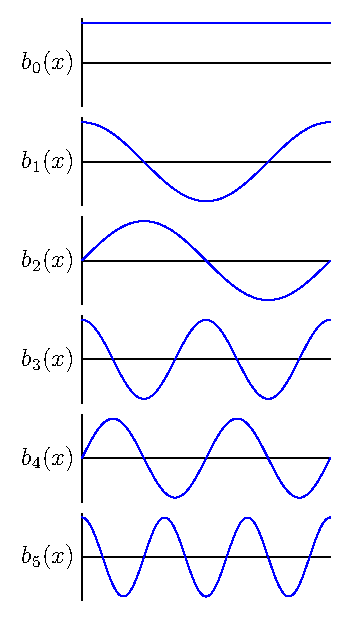
\includegraphics[width=0.9\linewidth]{fourier}\\
      \vspace*{1cm}
      \includegraphics[width=0.9\linewidth]{R3}
    \end{center}
  \end{minipage}
\end{PauseHighLight}

\end{slide}



%%%%%%%%%%%%%%%%%%%%%%% Next Slide %%%%%%%%%%%%%%%%%%%%%%%

\begin{slide}
\section[-1]{Algebraic Structure}

\begin{PauseHighLight}
  \begin{itemize}
  \item We have gone to these lengths as we want to show that many
    properties of vectors are shared by other objects (matrices,
    functions, etc.)\pause
  \item The notions of distance (geometry), norms (size of vectors) and
    inner products (angles between vectors) provides a very rich set
    of concepts\pause
  \item Vectors form the backbone of  objects we will use repeated in
    machine learning\pause
  \item The next piece of the jigsaw is to understand how we can
    transform these objects\pause
  \end{itemize}
\end{PauseHighLight}

\end{slide}

%%%%%%%%%%%%%%%%%%%%%%% Next Slide %%%%%%%%%%%%%%%%%%%%%%%
\Outline % Operators
%%%%%%%%%%%%%%%%%%%%%%% Next Slide %%%%%%%%%%%%%%%%%%%%%%%

\begin{slide}
\section{Operators}

\begin{PauseHighLight}
  \begin{itemize}
  \item In machine learning we are interested in transforming our input
    vectors into some output predictions\pause
  \item To accomplish this we will apply some mapping or operators on
    the vector $\mathcal{T}: \mathcal{V} \rightarrow \mathcal{V}'$\pause
  \item This says that $\mathcal{T}$ maps some object
    $\bm{x}\in\mathcal{V}$ to an object $\bm{y}=\mathcal{T}[\bm{x}]$ in
    a new vector space $\mathcal{V}'$\pause
  \item This new vector space may or may not be the same as the original
    vector space\pause
  \item Our objects may be any object in a vector space such as a
    function\pause
  \end{itemize}
\end{PauseHighLight}

\end{slide}

%%%%%%%%%%%%%%%%%%%%%%% Next Slide %%%%%%%%%%%%%%%%%%%%%%%

\begin{slide}
\section{Linear Operators}

\begin{PauseHighLight}
  \begin{itemize}
  \item Operators are in general very complicated, but a particular nice set
    of operators are linear operators\pause
  \item $\mathcal{T}$ is a linear operator if
    \begin{enumerate}
    \item $\mathcal{T}[a\,\bm{x}] = a\,\mathcal{T}[\bm{x}]$
    \item $\mathcal{T}[\bm{x} + \bm{y}] = \mathcal{T}[\bm{x}] +
      \mathcal{T}[\bm{y}]$\pause
    \end{enumerate}
  \item For normal vectors ($\bm{x}\in\mathbb{R}^n$) the most general linear operation is
    \begin{align*}
      \mathcal{T}[\bm{x}] = \mat{M}\,\bm{x}
    \end{align*}
  where $\mat{M}$ is a matrix\pause
  \end{itemize}
\end{PauseHighLight}

\end{slide}

%%%%%%%%%%%%%%%%%%%%%%% Next Slide %%%%%%%%%%%%%%%%%%%%%%%

\begin{slide}
\section[-2]{Matrix multiplication}

\begin{PauseHighLight}
  \begin{itemize}
  \item For an $\ell \times m$ matrix $\mat{A}$ and an $m \times n$
    matrix $\mat{B}$ we can compute the ($\ell\times n$) product, $\mat{C} =
    \mat{A}\,\mat{B}$, such that
    \begin{align*}
      C_{ij} = \sum_{k=1}^m A_{ik}\,B_{kj}\pause \hspace{2cm}
      \raisebox{-1cm}{\includegraphics[width=0.3\linewidth]{matrixMult}}
    \end{align*}
  \item Treating the vector $\bm{x}$ as a $n\times1$ matrix then
    \begin{align*}
      \bm{y} = \mat{A}\, \bm{x} \quad \Rightarrow \quad y_i = \sum_{j}
      M_{ij} x_j\pause \hspace{2cm}
      \raisebox{-1cm}{\includegraphics[width=0.27\linewidth]{matrixVector}}
    \end{align*}
  \item Using the same matrix notation we can define the inner product
    as
    \begin{align*}
      \langle \bm{x}, \bm{y} \rangle = \bm{x}^\tr \bm{y} = \sum_{i=1}^n
      x_i\,y_i \pause \hspace{2cm}
      \raisebox{-1cm}{\includegraphics[width=0.25\linewidth]{dotProduct}}
    \end{align*}
  \end{itemize}
\end{PauseHighLight}

\end{slide}

%%%%%%%%%%%%%%%%%%%%%%% Next Slide %%%%%%%%%%%%%%%%%%%%%%%

\begin{slide}
\section[-2]{Non-commutativity}
  
\begin{PauseHighLight}
  \begin{itemize}
  \item In general $\mat{A} \mat{B} \neq \mat{B} \mat{A}$\pause
    {\tiny
      \begin{align*}
      \begin{pmatrix}
        0 & -1 & 0 \\
        1 & 0 & 0 \\
        0 & 0 & 1
      \end{pmatrix} \,
        \begin{pmatrix}
        1 & 0 & 0 \\
        0 & 0 & -1 \\
        0 & 1 & 0
      \end{pmatrix}
                &=
                \begin{pmatrix}
                  0 & 0 & 1 \\
                  1 & 0 & 0 \\
                  0 & 1 &0
                \end{pmatrix}\pauseb
                , &
      \begin{pmatrix}
        1 & 0 & 0 \\
        0 & 0 & -1 \\
        0 & 1 & 0
      \end{pmatrix} \,
      \begin{pmatrix}
        0 & -1 & 0 \\
        1 & 0 & 0 \\
        0 & 0 & 1
      \end{pmatrix}
                &=
                \begin{pmatrix}
                  0 & -1 & 0 \\
                  0 & 0 & -1 \\
                  1 & 0 &0
                \end{pmatrix}\pauseb
      \end{align*}}
  \end{itemize}
\end{PauseHighLight}
\begin{center}
  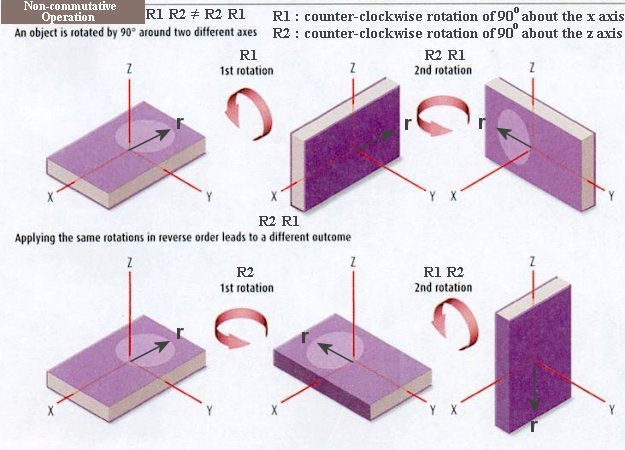
\includegraphics[width=0.6\linewidth]{nonAbelian}\pauseb
\end{center}
\end{slide}

%%%%%%%%%%%%%%%%%%%%%%% Next Slide %%%%%%%%%%%%%%%%%%%%%%%

\begin{slide}
  \section[-1]{Associativity of Mappings}

  \pb\pause\pauselevel{=1}
  \begin{center}
    \multipdf[width=\linewidth]{associativity}\pause
  \end{center}
  \begin{itemize}
  \item For all $\bm{x}$ we have $\mat{A}(\mat{B}\mat{C})\bm{x} =
    (\mat{A}\mat{B})\mat{C}\bm{x}$\pause
  \item This implies $\mat{A}(\mat{B}\mat{C}) = (\mat{A}\mat{B})\mat{C}$\pause
  \end{itemize}
\end{slide}



%%%%%%%%%%%%%%%%%%%%%%% Next Slide %%%%%%%%%%%%%%%%%%%%%%%

\begin{slide}
\section{Kernels}

\begin{PauseHighLight}
  \begin{itemize}
  \item The equivalent of a matrix for functions (i.e. a linear
    operator) is known as a kernel $K(x,y)$
    \begin{align*}
      g(x) = \mathcal{T}[f] = \int_{y\in\mathcal{I}} K(x,y)\, f(y) \,
      \dd y\pause
    \end{align*}
  \item Our domain does not need to be one dimensional, e.g.
    \begin{align*}
      g(\bm{x}) = \mathcal{T}[f] = \int_{\bm{y}\in\mathcal{I}}
      K(\bm{x},\bm{y})\, f(\bm{y}) \, \dd \bm{y}\pause
    \end{align*}
  \item We shall soon see examples of high-dimensional kernels\pause
  \end{itemize}
\end{PauseHighLight}

\end{slide}

%%%%%%%%%%%%%%%%%%%%%%% Next Slide %%%%%%%%%%%%%%%%%%%%%%%

\begin{slide}
\section[-1]{Kernels in Machine Learning}

\begin{PauseHighLight}
  \begin{itemize}
  \item Kernels are used heavily in machine learning\pause
  \item In kernel methods such as SVM, SVR, Kernel-PCA\pause
  \item They are also used in Gaussian Processes\pause
  \item In all these cases we consider symmetric, positive
    semi-definite kernels\pause
  \item Sometimes they can be interpreted as covariance between random functions
    \begin{align*}
      K(\bm{x},\bm{y})
      = \av[f\sim\mathcal{P}]{\left(\strut f(\bm{x})-\mu(\bm{x})\right)
      \left(\strut f(\bm{y})-\mu(\bm{y})\right)}\pause
    \end{align*}
  \end{itemize}
\end{PauseHighLight}


\end{slide}

%%%%%%%%%%%%%%%%%%%%%%% Next Slide %%%%%%%%%%%%%%%%%%%%%%%

\begin{slide}
\section[-2]{General Linear Mappings}

\pb\pause\pauselevel{=1}
\begin{itemize}
\item In general a linear operator will map vectors between different
  vector spaces\pauseh
\item E.g. $\mathbb{R}^3 \rightarrow \mathbb{R}^2$\pauseh\pauselevel{=1 =2}
  \begin{center}
    \multipdf[width=0.8\linewidth]{generalMap}\pause
  \end{center}
\end{itemize}


\end{slide}

%%%%%%%%%%%%%%%%%%%%%%% Next Slide %%%%%%%%%%%%%%%%%%%%%%%

\begin{slide}
\section{Square Matrices}

\begin{PauseHighLight}
  \begin{itemize}
  \item We will spend a lot of time on operators that map from a vector
    space onto itself $\mathcal{T}: \mathcal{V}\rightarrow\mathcal{V}$\pause
  \item For vectors in $\mathbb{R}^n$ such linear operators are
    represented by square matrices\pause
  \item When there is a one-to-one mapping then we have a unique inverse\pause
  \item We will study such mappings in detail in the next lecture\pause
  \end{itemize}
\end{PauseHighLight}

\end{slide}

%%%%%%%%%%%%%%%%%%%%%%% Next Slide %%%%%%%%%%%%%%%%%%%%%%%

\begin{slide}
\section{Summary}

\begin{PauseHighLight}
  \begin{itemize}
  \item We haven't covered much machine learning as
    such\pause---sorry\pauseb
  \item But mathematics is the language of machine learning and you have
    to get used to it\pause
  \item Mathematics is like programming, if you don't understand the
    syntax and you can't write it down then its meaningless\pause
  \item We've taken a high level view of inner product spaces and
    operator, this will pay us back later as we look at kernel
    methods\pause
  \end{itemize}
\end{PauseHighLight}

\end{slide}


%%% Local Variables:
%%% TeX-master: "lectures"
%%% End:
